%\pdfoutput=0
\documentclass[twocolumn]{article}
\usepackage{graphicx}
\usepackage{hyperref}
\usepackage{amsmath}
\title{An example of using \LaTeX \ and Gnuplot: Euler spiral}
\author{Lukas Martin Wick}
\begin{document}
\maketitle

An 'Euler spiral' is a curve whose curvature changes linearly with its curve length 
(the curvature of a circular curve is equal to the reciprocal of the radius). 
Euler spirals are also commonly referred to as 'spiros', 'clothoids', or 'Cornu spirals'.

Euler spirals have applications to diffraction computations. They are also widely used as transition curves in railroad engineering/highway engineering
for connecting and transitioning the geometry between a tangent and a circular curve. 
A similar application is also found in photonic integrated circuits. The principle of linear 
variation of the curvature of the transition curve between a tangent and a circular curve defines the geometry of the Euler spiral: 

\begin{itemize}
    \item Its curvature begins with zero at the straight section (the tangent) and increases linearly with its curve length.
    \item Where the Euler spiral meets the circular curve, its curvature becomes equal to that of the latter.
\end{itemize}

Normalized Euler spirals can be expressed as:
\begin{align}
    x &= \int_0^L \cos s^2 ds \\
    y &= \int_0^L \sin s^2 ds
\end{align}
The above is from \url{https://en.wikipedia.org/wiki/Euler_spiral}.
A plot of the normalized Euler spirals can be seen in figure \ref{fig:eulerSpirals}
\begin{figure}[]
    \centering
% GNUPLOT: LaTeX picture with Postscript
\begingroup
  \makeatletter
  \providecommand\color[2][]{%
    \GenericError{(gnuplot) \space\space\space\@spaces}{%
      Package color not loaded in conjunction with
      terminal option `colourtext'%
    }{See the gnuplot documentation for explanation.%
    }{Either use 'blacktext' in gnuplot or load the package
      color.sty in LaTeX.}%
    \renewcommand\color[2][]{}%
  }%
  \providecommand\includegraphics[2][]{%
    \GenericError{(gnuplot) \space\space\space\@spaces}{%
      Package graphicx or graphics not loaded%
    }{See the gnuplot documentation for explanation.%
    }{The gnuplot epslatex terminal needs graphicx.sty or graphics.sty.}%
    \renewcommand\includegraphics[2][]{}%
  }%
  \providecommand\rotatebox[2]{#2}%
  \@ifundefined{ifGPcolor}{%
    \newif\ifGPcolor
    \GPcolortrue
  }{}%
  \@ifundefined{ifGPblacktext}{%
    \newif\ifGPblacktext
    \GPblacktexttrue
  }{}%
  % define a \g@addto@macro without @ in the name:
  \let\gplgaddtomacro\g@addto@macro
  % define empty templates for all commands taking text:
  \gdef\gplbacktext{}%
  \gdef\gplfronttext{}%
  \makeatother
  \ifGPblacktext
    % no textcolor at all
    \def\colorrgb#1{}%
    \def\colorgray#1{}%
  \else
    % gray or color?
    \ifGPcolor
      \def\colorrgb#1{\color[rgb]{#1}}%
      \def\colorgray#1{\color[gray]{#1}}%
      \expandafter\def\csname LTw\endcsname{\color{white}}%
      \expandafter\def\csname LTb\endcsname{\color{black}}%
      \expandafter\def\csname LTa\endcsname{\color{black}}%
      \expandafter\def\csname LT0\endcsname{\color[rgb]{1,0,0}}%
      \expandafter\def\csname LT1\endcsname{\color[rgb]{0,1,0}}%
      \expandafter\def\csname LT2\endcsname{\color[rgb]{0,0,1}}%
      \expandafter\def\csname LT3\endcsname{\color[rgb]{1,0,1}}%
      \expandafter\def\csname LT4\endcsname{\color[rgb]{0,1,1}}%
      \expandafter\def\csname LT5\endcsname{\color[rgb]{1,1,0}}%
      \expandafter\def\csname LT6\endcsname{\color[rgb]{0,0,0}}%
      \expandafter\def\csname LT7\endcsname{\color[rgb]{1,0.3,0}}%
      \expandafter\def\csname LT8\endcsname{\color[rgb]{0.5,0.5,0.5}}%
    \else
      % gray
      \def\colorrgb#1{\color{black}}%
      \def\colorgray#1{\color[gray]{#1}}%
      \expandafter\def\csname LTw\endcsname{\color{white}}%
      \expandafter\def\csname LTb\endcsname{\color{black}}%
      \expandafter\def\csname LTa\endcsname{\color{black}}%
      \expandafter\def\csname LT0\endcsname{\color{black}}%
      \expandafter\def\csname LT1\endcsname{\color{black}}%
      \expandafter\def\csname LT2\endcsname{\color{black}}%
      \expandafter\def\csname LT3\endcsname{\color{black}}%
      \expandafter\def\csname LT4\endcsname{\color{black}}%
      \expandafter\def\csname LT5\endcsname{\color{black}}%
      \expandafter\def\csname LT6\endcsname{\color{black}}%
      \expandafter\def\csname LT7\endcsname{\color{black}}%
      \expandafter\def\csname LT8\endcsname{\color{black}}%
    \fi
  \fi
    \setlength{\unitlength}{0.0500bp}%
    \ifx\gptboxheight\undefined%
      \newlength{\gptboxheight}%
      \newlength{\gptboxwidth}%
      \newsavebox{\gptboxtext}%
    \fi%
    \setlength{\fboxrule}{0.5pt}%
    \setlength{\fboxsep}{1pt}%
\begin{picture}(7200.00,4320.00)%
    \gplgaddtomacro\gplbacktext{%
      \csname LTb\endcsname%
      \put(2009,595){\makebox(0,0)[r]{\strut{}$-1$}}%
      \csname LTb\endcsname%
      \put(2009,947){\makebox(0,0)[r]{\strut{}$-0.8$}}%
      \csname LTb\endcsname%
      \put(2009,1299){\makebox(0,0)[r]{\strut{}$-0.6$}}%
      \csname LTb\endcsname%
      \put(2009,1651){\makebox(0,0)[r]{\strut{}$-0.4$}}%
      \csname LTb\endcsname%
      \put(2009,2003){\makebox(0,0)[r]{\strut{}$-0.2$}}%
      \csname LTb\endcsname%
      \put(2009,2355){\makebox(0,0)[r]{\strut{}$0$}}%
      \csname LTb\endcsname%
      \put(2009,2707){\makebox(0,0)[r]{\strut{}$0.2$}}%
      \csname LTb\endcsname%
      \put(2009,3059){\makebox(0,0)[r]{\strut{}$0.4$}}%
      \csname LTb\endcsname%
      \put(2009,3411){\makebox(0,0)[r]{\strut{}$0.6$}}%
      \csname LTb\endcsname%
      \put(2009,3763){\makebox(0,0)[r]{\strut{}$0.8$}}%
      \csname LTb\endcsname%
      \put(2009,4115){\makebox(0,0)[r]{\strut{}$1$}}%
      \csname LTb\endcsname%
      \put(2111,409){\makebox(0,0){\strut{}$-1$}}%
      \csname LTb\endcsname%
      \put(2463,409){\makebox(0,0){\strut{}$-0.8$}}%
      \csname LTb\endcsname%
      \put(2815,409){\makebox(0,0){\strut{}$-0.6$}}%
      \csname LTb\endcsname%
      \put(3167,409){\makebox(0,0){\strut{}$-0.4$}}%
      \csname LTb\endcsname%
      \put(3519,409){\makebox(0,0){\strut{}$-0.2$}}%
      \csname LTb\endcsname%
      \put(3871,409){\makebox(0,0){\strut{}$0$}}%
      \csname LTb\endcsname%
      \put(4223,409){\makebox(0,0){\strut{}$0.2$}}%
      \csname LTb\endcsname%
      \put(4575,409){\makebox(0,0){\strut{}$0.4$}}%
      \csname LTb\endcsname%
      \put(4927,409){\makebox(0,0){\strut{}$0.6$}}%
      \csname LTb\endcsname%
      \put(5279,409){\makebox(0,0){\strut{}$0.8$}}%
      \csname LTb\endcsname%
      \put(5631,409){\makebox(0,0){\strut{}$1$}}%
    }%
    \gplgaddtomacro\gplfronttext{%
      \csname LTb\endcsname%
      \put(1406,2355){\rotatebox{-270}{\makebox(0,0){\strut{}$y$}}}%
      \csname LTb\endcsname%
      \put(3871,130){\makebox(0,0){\strut{}$x$}}%
      \csname LTb\endcsname%
      \put(3437,3948){\makebox(0,0)[r]{\strut{}Euler spiral}}%
    }%
    \gplbacktext
    \put(0,0){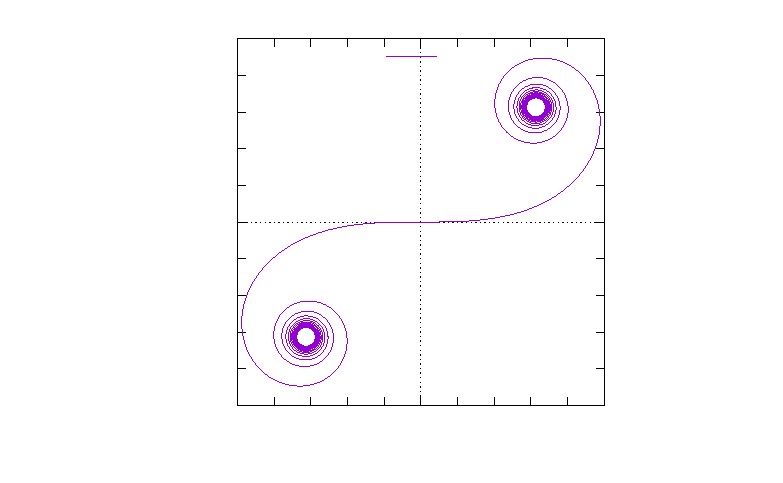
\includegraphics{plot-eulerSpiral}}%
    \gplfronttext
  \end{picture}%
\endgroup

\caption{Illustration of the Euler spiral function.}
\label{fig:eulerSpirals}
\end{figure}

\end{document}
